\documentclass[11pt, letterpaper]{article}

\usepackage[margin=1in]{geometry}
\usepackage[T1]{fontenc}
\usepackage[utf8]{inputenc}
\usepackage{amsmath}
\usepackage{amssymb}
\usepackage{booktabs}
\usepackage{array}
\usepackage{caption}
\usepackage{hyperref}
\usepackage{natbib}
\usepackage{setspace}
\usepackage{tikz}
\usepackage{xcolor}
\usetikzlibrary{arrows.meta, positioning}

\hypersetup{colorlinks=true, linkcolor=blue, citecolor=blue, urlcolor=blue}
\onehalfspacing

\definecolor{qNavy}{RGB}{18,45,88}
\definecolor{qBlue}{RGB}{37,112,165}
\definecolor{qGold}{RGB}{201,155,45}
\definecolor{qGray}{RGB}{90,96,105}
\definecolor{qLight}{RGB}{232,238,245}

\title{\textbf{Predicting Asset Returns with a Structured Strategy Space}\\
\large A Two-Layer Framework for Adaptive Trading Signals}
\author{Joon Jeremy Chun}
\date{May 2026}

\begin{document}

\maketitle

\begin{abstract}
This report studies whether a structured representation of trading signals can improve near-future asset-return prediction. The project focuses on GLD and evaluates a two-layer architecture: a fixed strategy-space layer that maps prices into parameterized trading signals, followed by a regularized linear model that predicts 130-day forward returns. A rolling forward test over 2020--2025 compares three stages: a single best strategy, a constrained ensemble, and a machine-learning-guided predictor. The ML-guided stage produces the strongest annual strategy return in every evaluation year and remains approximately flat in weak benchmark years. The results suggest that the value of the framework comes from aligning the strategy representation with the prediction horizon and updating the model as market regimes change.
\end{abstract}

\section{Introduction}

Financial time series prediction is difficult because the data are noisy, nonstationary, and limited in sample size. A short training window can overfit idiosyncratic price movement, while a long window can include outdated regimes. This tension is especially important for trading systems, where each decision must use only information available at the time of prediction.

The question addressed in this project is whether a structured collection of trading strategies can be used as a predictive feature space. Instead of feeding raw prices or arbitrary indicators into a machine learning model, each feature is the output of a parameterized trading rule. Over a training window of length $T$, each signal is a vector in $\mathbb{R}^T$, and a family of strategies spans a design matrix.

The central hypothesis is that this representation makes a short-window prediction problem more stable. Domain knowledge constructs meaningful candidate signals; regularized regression selects and combines them. Thus, the nonlinear price transformation is fixed by trading theory and grid search, while the linear prediction layer is learned adaptively.

The project is evaluated on GLD from 2020 through 2024. The prediction target is the 130-day forward return, and the model is re-estimated monthly using the preceding one-year window. The report follows a standard scientific structure: background literature, methods, results, and discussion. A separate reflection is included at the end.

\section{Background}

Quantitative trading systems often combine many ``alpha'' signals, where each signal is a candidate predictor of future return. \citet{kakushadze2015} formulate alpha combination as a bounded regression problem. This project uses a related view: strategy signals are treated as basis functions, but the learned combination predicts a future return target rather than only optimizing realized historical return.

The statistical motivation comes from sparse regression. The Lasso \citep{tibshirani1996} adds an $\ell_1$ penalty to least squares regression, shrinking many coefficients exactly to zero. This is useful when the number of candidate predictors is large relative to the number of training observations. In this project, the training window contains approximately one year of daily observations, while the strategy matrix may contain dozens of candidate signals. Regularization is therefore necessary to prevent the learned linear layer from fitting noise.

Together, these ideas motivate an interpretable model that is adaptive but constrained enough to be estimated on a short rolling window.

\section{Methods}

\subsection{Strategy-Space Construction}

Let $p(t)$ denote the GLD price series. A trading strategy with parameter vector $\theta$ maps historical prices into a daily signal
\[
    s_{\theta}(t) \in [-1,1],
\]
where positive values indicate long exposure and values near zero indicate weak or no exposure. Over $T$ training days, this strategy produces a vector
\[
    \mathbf{s}_{\theta} = (s_{\theta}(1),\ldots,s_{\theta}(T))^\top \in \mathbb{R}^T.
\]
The collection of such vectors forms a strategy space. In this project, four strategy families are used: adaptive price bands, moving-average crossovers, adaptive volatility bands, and a candle-volume fear-greed signal.

For each monthly anchor date, every strategy family is searched over a parameter grid using only the preceding one-year window. Let $\tau$ denote an anchor date and $W_\tau$ the one-year training window ending at $\tau$. For a strategy family $f$ with parameter grid $\Theta_f$, each $\theta\in\Theta_f$ produces a signal vector $\mathbf{s}_{f,\theta}$ on $W_\tau$. The grid-search layer evaluates
\[
    R_\tau(f,\theta)
    =
    \sum_{t\in W_\tau} s_{f,\theta}(t)\, r_{t+1},
\]
where $r_{t+1}$ is the next-day realized asset return. If candidate strategy vectors are collected as columns of $A_{f,\tau}$, the ensemble signal is
\[
    \mathbf{z}_{\tau}=A_{f,\tau}\mathbf{x},
    \qquad
    \mathbf{x}\geq 0,\quad \mathbf{1}^{\top}\mathbf{x}=1,
\]
with $\mathbf{x}$ chosen to maximize realized return on $W_\tau$. Thus, the first layer is a selection procedure, not a future-return prediction model.

The top $N$ parameter settings per family are selected by $R_\tau(f,\theta)$. These selected signals are then concatenated into a design matrix
\[
    A = [\mathbf{s}_{1}, \mathbf{s}_{2}, \ldots, \mathbf{s}_{4N}]
    \in \mathbb{R}^{T \times 4N}.
\]
The main experiments use $N=10$, producing 40 strategy columns. This matrix is recomputed at each anchor date, so the strategy subspace is allowed to adapt over time.

\begin{figure}[htbp]
\centering
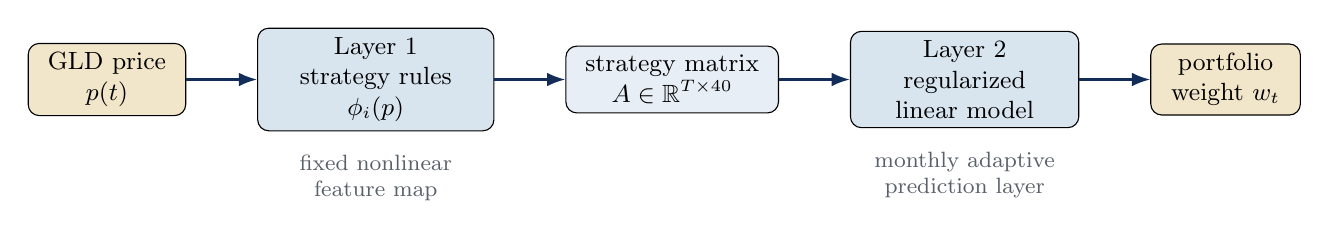
\begin{tikzpicture}[
  node distance=0.7cm and 0.9cm,
  box/.style={draw, rounded corners, align=center, minimum height=0.75cm, font=\small},
  arrow/.style={-{Latex}, thick, qNavy}
]
  \node[box, fill=qGold!25, minimum width=2.0cm] (price) {GLD price\\$p(t)$};
  \node[box, fill=qBlue!18, right=of price, minimum width=3.0cm] (layer1) {Layer 1\\strategy rules\\$\phi_i(p)$};
  \node[box, fill=qLight, right=of layer1, minimum width=2.7cm] (matrix) {strategy matrix\\$A\in\mathbb{R}^{T\times 40}$};
  \node[box, fill=qBlue!18, right=of matrix, minimum width=2.9cm] (layer2) {Layer 2\\regularized\\linear model};
  \node[box, fill=qGold!25, right=of layer2, minimum width=1.9cm] (weight) {portfolio\\weight $w_t$};
  \draw[arrow] (price) -- (layer1);
  \draw[arrow] (layer1) -- (matrix);
  \draw[arrow] (matrix) -- (layer2);
  \draw[arrow] (layer2) -- (weight);
  \node[below=0.18cm of layer1, font=\footnotesize, color=qGray, align=center] {fixed nonlinear\\feature map};
  \node[below=0.18cm of layer2, font=\footnotesize, color=qGray, align=center] {monthly adaptive\\prediction layer};
\end{tikzpicture}
\caption{Conceptual architecture of the two-layer strategy-space model. The first layer converts price history into interpretable strategy signals. The second layer learns a regularized linear predictor of the 130-day forward return and converts the prediction into a long-only portfolio weight.}
\label{fig:architecture}
\end{figure}

\subsection{Prediction Model and Horizon Selection}

The second layer changes the objective from maximizing realized training-window return to predicting a future return. For candidate horizon $h$,
\[
    y_t^{(h)} = \frac{p(t+h)-p(t)}{p(t)}.
\]
Given the strategy matrix $A_\tau$ constructed from the top strategy vectors at anchor $\tau$, the machine-learning model is written as
\[
    \mathbf{y}^{(h)} = A_\tau\boldsymbol{\beta}^{(h)} + \boldsymbol{\varepsilon},
    \qquad
    \hat{\mathbf{y}}^{(h)} = A_\tau\hat{\boldsymbol{\beta}}^{(h)}.
\]
Here $\mathbf{y}^{(h)}$ records the future $h$-day return following each row of the strategy matrix. The first layer asks which strategy signals were useful in the recent regime; the second asks which combination predicts future returns.

Ridge, Lasso, and Elastic Net models are considered. In general form, the fitted coefficient vector solves
\[
  \hat{\boldsymbol{\beta}}^{(h)}
  =
  \arg\min_{\boldsymbol{\beta}}
  \left[
    \frac{1}{T}\|A_\tau\boldsymbol{\beta}-\mathbf{y}^{(h)}\|_2^2
    + \lambda_1\|\boldsymbol{\beta}\|_1
    + \lambda_2\|\boldsymbol{\beta}\|_2^2
  \right].
\]
Ridge uses only the $\ell_2$ penalty, Lasso uses only the $\ell_1$ penalty, and Elastic Net uses both. Hyperparameters are selected by cross-validated mean squared error within the training window.

The horizon $h$ was not assumed in advance. The project scanned $h=1,2,\ldots,260$ and found two candidate regions: near 45 trading days and near 130 trading days. The final model uses $h=130$ because it was more stable across regimes and close to six months, matching the temporal scale of the Layer 1 selection process.

The predicted return is converted into a long-only weight $w_t\in[0,1]$ by scaling positive predictions and clipping negative predictions to zero, so the model can reduce exposure when uncertainty is high.

\subsection{Evaluation Design}

Three stages are evaluated. Stage A deploys the single best grid-search strategy. Stage B combines selected strategies with constrained weights optimized on the selection window. Stage C uses the regularized prediction model above. The stages isolate the value of moving from a single signal, to an ensemble, to an explicitly predictive model.

The validation protocol is a rolling forward test. At each monthly anchor date, all strategy selection and model fitting use only the previous year of data. The fitted model is then evaluated out of sample. The primary evaluation period is 2020--2025. This design prevents look-ahead bias because no future prices are used in strategy selection, model fitting, or hyperparameter choice at the anchor date.

Performance is reported as annual return and average capital exposure. Because the strategy often holds less than full exposure, capital efficiency is also reported:
\[
    \text{capital efficiency}
    =
    \frac{\text{strategy return}}{\text{average exposure}}.
\]
This measures return per dollar of deployed capital and is useful for comparing a partial-exposure strategy with buy-and-hold.

\section{Results}

\subsection{Three-Stage Comparison}

The three-stage comparison shows a consistent improvement from single strategies to the machine-learning-guided predictor. Table~\ref{tab:stage-results} reports annual returns and exposures for GLD from 2020 through 2025. Stage C has the highest return among the three strategy stages in every year. The difference is especially clear in 2024, where Stage A returns 5.9\%, Stage B returns 8.0\%, and Stage C returns 16.4\%.

\begin{table}[htbp]
\centering
\caption{Annual GLD forward-test results by stage. Values are return / average exposure. Buy-and-hold is shown as annual GLD return with full exposure. Years denote the forward evaluation year, not the training year; each monthly model is trained on the preceding one-year window.}
\label{tab:stage-results}
\small
\begin{tabular}{lrrrr}
\toprule
Year & Buy-and-hold & Stage A & Stage B & Stage C \\
\midrule
2020 & $+23.9\%$ & $+4.4\%$ / 27\% & $+6.4\%$ / 32\% & $\mathbf{+10.9\%}$ / 57\% \\
2021 & $-6.2\%$  & $+0.3\%$ / 25\% & $+0.3\%$ / 25\% & $\mathbf{+0.8\%}$ / 29\% \\
2022 & $+0.8\%$  & $-0.9\%$ / 46\% & $-2.3\%$ / 42\% & $\mathbf{-0.2\%}$ / 31\% \\
2023 & $+11.8\%$ & $+1.6\%$ / 25\% & $+2.0\%$ / 23\% & $\mathbf{+4.0\%}$ / 32\% \\
2024 & $+27.0\%$ & $+5.9\%$ / 21\% & $+8.0\%$ / 29\% & $\mathbf{+16.4\%}$ / 65\% \\
2025 & $+61.5\%$ & $+21.4\%$ / 40\% & $+21.4\%$ / 40\% & $\mathbf{+34.7\%}$ / 65\% \\
\bottomrule
\end{tabular}
\end{table}

Stage C is not simply increasing exposure indiscriminately. In 2021, GLD declined by 6.2\%, while Stage C remained positive with only 29\% average exposure; in 2022, it lost less than the simpler stages. Its raw return does not usually match buy-and-hold because the model is often partially invested, but its capital efficiency is close to the fully invested benchmark in strong years and better in weak years. This is meaningful because the model is trained to predict $y_t^{(130)}$, not to directly maximize realized portfolio return.

\begin{figure}[htbp]
\centering
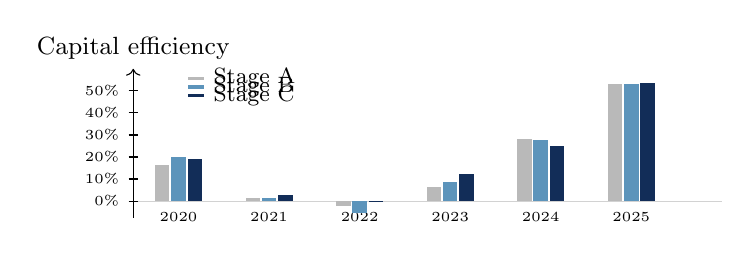
\begin{tikzpicture}[xscale=1.15, yscale=2.8]
  \draw[gray!35] (0.5,0) -- (7.0,0);
  \draw[->] (0.5,-0.075) -- (0.5,0.60) node[above,font=\small] {Capital efficiency};
  \foreach \v/\lbl in {0/0\%,0.10/10\%,0.20/20\%,0.30/30\%,0.40/40\%,0.50/50\%} {
    \draw (0.45,\v) -- (0.55,\v);
    \node[left,font=\tiny] at (0.45,\v) {\lbl};
  }
  \foreach \x/\yr in {1/2020,2/2021,3/2022,4/2023,5/2024,6/2025} {
    \node[below,font=\tiny] at (\x,-0.01) {\yr};
  }
  \foreach \x/\a/\b/\c in {
    1/0.163/0.200/0.191,
    2/0.012/0.012/0.028,
    3/-0.020/-0.055/-0.006,
    4/0.064/0.087/0.125,
    5/0.281/0.276/0.252,
    6/0.531/0.531/0.536
  } {
    \fill[gray!55]  (\x-0.26,0) rectangle (\x-0.10,\a);
    \fill[qBlue!75] (\x-0.08,0) rectangle (\x+0.08,\b);
    \fill[qNavy]   (\x+0.10,0) rectangle (\x+0.26,\c);
  }
  \fill[gray!55] (1.10,0.55) rectangle (1.28,0.565);
  \node[right,font=\footnotesize] at (1.28,0.557) {Stage A};
  \fill[qBlue!75] (1.10,0.51) rectangle (1.28,0.525);
  \node[right,font=\footnotesize] at (1.28,0.517) {Stage B};
  \fill[qNavy] (1.10,0.47) rectangle (1.28,0.485);
  \node[right,font=\footnotesize] at (1.28,0.477) {Stage C};
\end{tikzpicture}
\caption{Capital efficiency by stage and year. Stage C produces the strongest efficiency in most years and avoids the larger negative efficiency observed in Stage B during 2022.}
\label{fig:stage-efficiency}
\end{figure}

\subsection{Prediction Horizon}

The strongest result is the importance of matching the prediction target to the scale of the strategy features. A shorter 45-day target was also evaluated. Although it performs well in strong upward markets, it is less stable in adverse years. Figure~\ref{fig:horizon} compares capital efficiency for the 130-day and 45-day models.

\begin{figure}[htbp]
\centering
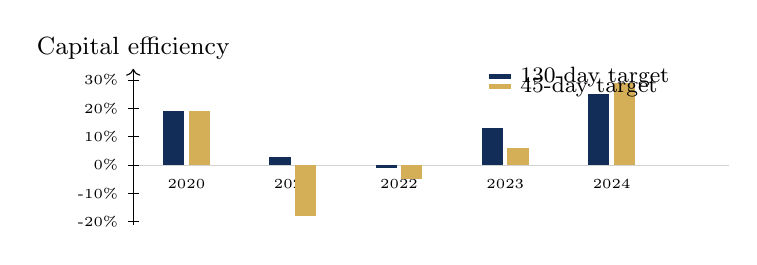
\begin{tikzpicture}[xscale=1.35, yscale=3.6]
  \draw[gray!35] (0.5,0) -- (6.1,0);
  \draw[->] (0.5,-0.21) -- (0.5,0.34) node[above,font=\small] {Capital efficiency};
  \foreach \v/\lbl in {-0.20/-20\%,-0.10/-10\%,0/0\%,0.10/10\%,0.20/20\%,0.30/30\%} {
    \draw (0.45,\v) -- (0.55,\v);
    \node[left,font=\tiny] at (0.45,\v) {\lbl};
  }
  \foreach \x/\yr in {1/2020,2/2021,3/2022,4/2023,5/2024} {
    \node[below,font=\tiny] at (\x,-0.015) {\yr};
  }
  \foreach \x/\hA/\hB in {
    1/0.19/0.19,
    2/0.03/-0.18,
    3/-0.01/-0.05,
    4/0.13/0.06,
    5/0.25/0.29
  } {
    \fill[qNavy]   (\x-0.22,0) rectangle (\x-0.02,\hA);
    \fill[qGold!80] (\x+0.02,0) rectangle (\x+0.22,\hB);
  }
  \fill[qNavy] (3.85,0.305) rectangle (4.05,0.32);
  \node[right,font=\footnotesize] at (4.05,0.312) {130-day target};
  \fill[qGold!80] (3.85,0.27) rectangle (4.05,0.285);
  \node[right,font=\footnotesize] at (4.05,0.277) {45-day target};
\end{tikzpicture}
\caption{Capital efficiency for 130-day and 45-day prediction targets. The 45-day target performs well in 2024 but fails sharply in 2021. The 130-day target is more stable across regimes.}
\label{fig:horizon}
\end{figure}

This pattern supports the feature-target alignment hypothesis: Layer 1 selects strategy parameters using approximately six months of performance information, and 130 trading days is approximately six months. A much shorter target asks six-month features to predict a different time scale.

\subsection{Model Training and Live System}

At each anchor date, grid search, strategy selection, model fitting, and cross-validation used only historical data, preventing label or normalization leakage. The pipeline was also implemented as a live paper-trading system: a Raspberry Pi fetches the latest GLD price, computes the target weight, and records the signal. Code for the analysis and deployment pipeline is maintained in a public repository \citep{chun2026repo}.

\section{Discussion and Conclusions}

The strategy-space formulation provides a useful way to structure a difficult prediction problem. Layer 1 encodes domain knowledge into interpretable signals, reducing the burden on a short-window statistical model; Layer 2 learns a sparse or regularized combination of those signals.

The three-stage comparison clarifies the source of the improvement. The single-strategy baseline is too narrow: it captures only one type of price behavior. The constrained ensemble adds diversification, but it still optimizes past return rather than directly predicting future return. Stage C changes the objective. It asks which combination of strategy signals best predicts the forward return, and it updates that relationship monthly. This explains why Stage C improves on Stage B even though both use the same general strategy space.

The exposure pattern also motivates a future multi-asset version. The model should reduce exposure when prediction is uncertain and increase exposure when the signal is strong. The GLD results are consistent with this behavior: exposure is low in weaker years and rises in the strong 2024 regime. In a portfolio setting, idle GLD capital could be redeployed to another asset with a stronger signal.

The most important empirical finding is the role of prediction horizon. The 130-day target is more stable than the 45-day target because it is aligned with the window used to evaluate and select the strategy features. This finding is useful beyond the specific GLD experiment: in a two-layer model, the prediction target should be chosen to match the temporal scale of the features generated by the first layer.

Several limitations remain. The project focuses on one asset; transaction costs, slippage, and live execution constraints are not fully modeled; and the strategy families are manually specified. The five-year evaluation should therefore be interpreted as promising rather than definitive.

Future work should extend the framework to multiple assets, evaluate transaction costs, and compare the linear prediction layer with nonlinear models under the same rolling validation design.

A second extension is to add a third layer based on Sparse Identification of Nonlinear Dynamics (SINDy). The current prediction layer is linear in the selected strategy signals:
\[
    \hat{y}=A\hat{\beta}.
\]
This assumes that each signal contributes proportionally to predicted return. A richer model could construct nonlinear candidate functions,
\[
    \Theta(A)
    =
    [A,\ A^{\circ 2},\ A^{\circ 3},\ A_iA_j,\ \ldots],
\]
and use sparse regression to identify useful transformations. In trading terms, this asks whether exposure should scale linearly with the signal or whether a nonlinear activation, such as weak response to small signals and stronger response to large signals, is more appropriate.

Overall, the project shows that a structured strategy space, combined with regularized prediction and rolling validation, can produce an interpretable adaptive trading framework. The strongest evidence is not only that Stage C has better annual returns than the simpler stages, but that its behavior is consistent with the intended design: it increases exposure when predicted return is favorable and reduces exposure in weaker regimes.

\clearpage
\bibliographystyle{plainnat}
\bibliography{references}

\clearpage
\section*{Reflection}

This project surprised me because the most interesting part was not the trading result itself, but the process of turning a messy trading idea into a precise mathematical question. At the beginning, I was mostly thinking about whether I could build a strategy that made money. By the end, the better question was whether strategy outputs could be treated as a structured feature space for prediction.

This also changed how I think about machine learning for markets. When I first learned machine learning and deep learning, my team and I tried to predict the stock market by adding more features. The problem was that more features require more data, but in financial markets, using more historical data can introduce older regimes where the market narrative was different. If I instead reduce the window to focus on the current regime, the data become too small and noisy for a flexible model. This class helped me see that the answer is not always to make the model larger. Methods such as Lasso and regularized model selection gave me a way to think about reducing noise and selecting structure. In this project, replacing many arbitrary raw features with strategy-based features felt like a real shift in how I approach prediction.

The hardest part was being honest about validation. In financial data, it is very easy to accidentally let the future leak into the past. I had to keep checking whether each model decision used only information that would have been available at the anchor date. That made the project slower, but it also made the final results feel more meaningful.

The most surprising result was the 130-day horizon. I expected shorter horizons to react faster and therefore work better, but the 45-day model was much less stable. The explanation that made the most sense was feature-target alignment: the strategy features were selected using a roughly six-month window, so they were naturally better at predicting a roughly six-month target. That was a real research moment for me because the result forced me to understand the model architecture more deeply.

If I could do the project again, I would start the multi-asset version earlier. A single-asset strategy leaves a lot of capital idle, and that idle capital is probably where the next version of the project becomes interesting. I also learned that I work best when I turn broad goals into falsifiable questions. ``Can this model predict GLD better?'' was too vague. ``Does a 130-day target outperform a 45-day target under the same rolling validation protocol?'' was a question I could actually answer.

\end{document}
